\clearpage
\section{Demo Proposal}
\label{sec:demo}

The goal of our demonstration
is to illustrate the basic concepts of the Bloom programming language and the
program analysis techniques it supports for reasoning about consistency and
coordination in distributed programs.  We will demonstrate how to use Bloom to
develop several variants of a distributed shopping cart system, similar to the
case study described in Section~\ref{sec:case}.  The demo will involve
on-the-fly coding in Bloom, graphical representations of our program analysis
techniques, and graphical visualizations of the communication behavior in live
distributed services.

Although our Bloom code is currently running on Amazon EC2, we are concerned
about connectivity at Asilomar and hence plan to run our demo on a local-area
cluster of laptops.

We will begin by developing the destructive and disorderly variants of the
shopping cart example, initially without any coordination logic. We will run
these programs on our cluster, with one laptop as the client---submitting
requests to add or remove items from the cart---and the rest of the laptops as
server replicas (Figure~\ref{fig:demoarch}).  The client will dispatch each request to a random server
replica.  For demonstration purposes, we will interpose a \emph{demonic}
message delivery module, which operates at each server replica and delivers
messages in a random ``bad'' order (e.g., deletions before insertions,
checkouts before all insertions and deletions).

We will display a trace of the cart's execution in real time by visualizing the
messages sent by the client and received by each server replica, in the order
they are sent or received, and explain the potential hazards associated with
different orders. We will then apply our points-of-order program analysis in a
graphical form, and show how this technique identifies the possible message
ordering inconsistencies we have already demonstrated experimentally.

Finally, following the recommendations of the program analysis tool, we will
add coordination logic to the two shopping cart variants, verify consistency of
the result in our analysis tool, and run the modified code on the cluster of
laptops. We will benchmark the performance of the modified shopping cart
programs and visualize the results, demonstrating how the increased
coordination in the destructive shopping cart implementation results in reduced
performance. To ensure that this effect is visible, as it would be in a
distributed cloud environment, we need to ensure realistic latencies between
the laptops.  The wireless spectrum in Asilomar's conference room may be
sufficiently congested to serve this purpose.  Alternatively, we may interpose
a message delivery module to introduce delay.

\begin{figure}[t]
\centering
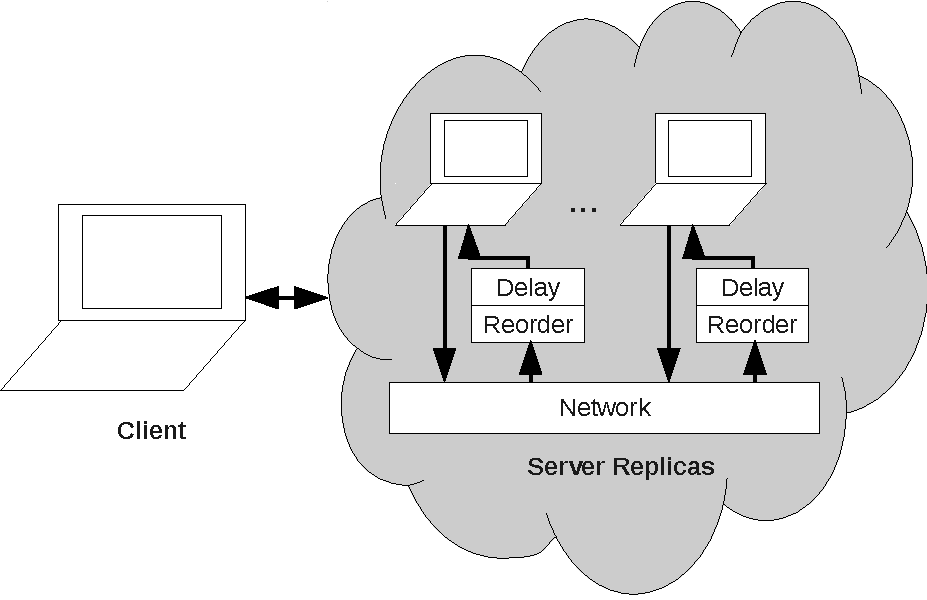
\includegraphics[width=0.9\linewidth]{fig/demoarch.pdf}
\caption{Demo architecture.}
\label{fig:demoarch}
\end{figure}

%may need to bring our own networking equipment and instrument it to add the
%appropriate amount of latency.
